\chapter{Training and evaluation}

The best practice on evaluating the classifier model's performance is to simply compare the number of matching labels evaluated on a completely disjunct set of samples from the training set.
However in our case it was not so trivial to score different methods, since by simply answering \textit{normal} to every sample would yield 50+\% success rate, therefore it would be less representative.

\section{Confusion matrix}
Instead we are using an extended version of precision-recall evaluation, namely we apply a \textit{confusion matrix}, where every row represents a histogram of the correct label, and every column represents the predictions of our model. The diagonal elements show how many labels match, but it preserves the distribution between classes.
Using this method, we can easily track down when a training routine collapses, and the network is only using a few of the available classes. When the diagonal elements over number the off-diagonals, then the network has been succesfully trained. For examples of the confusion matrix see Figure \ref{fig:confmatrix}.
By reducing the matrix to a single scalar defined on the website of AF Challenge, we get an accuracy value, which tells us the exact score we would obtain by submitting an official entry on behalf of our research group.

\begin{figure}
  \centering
  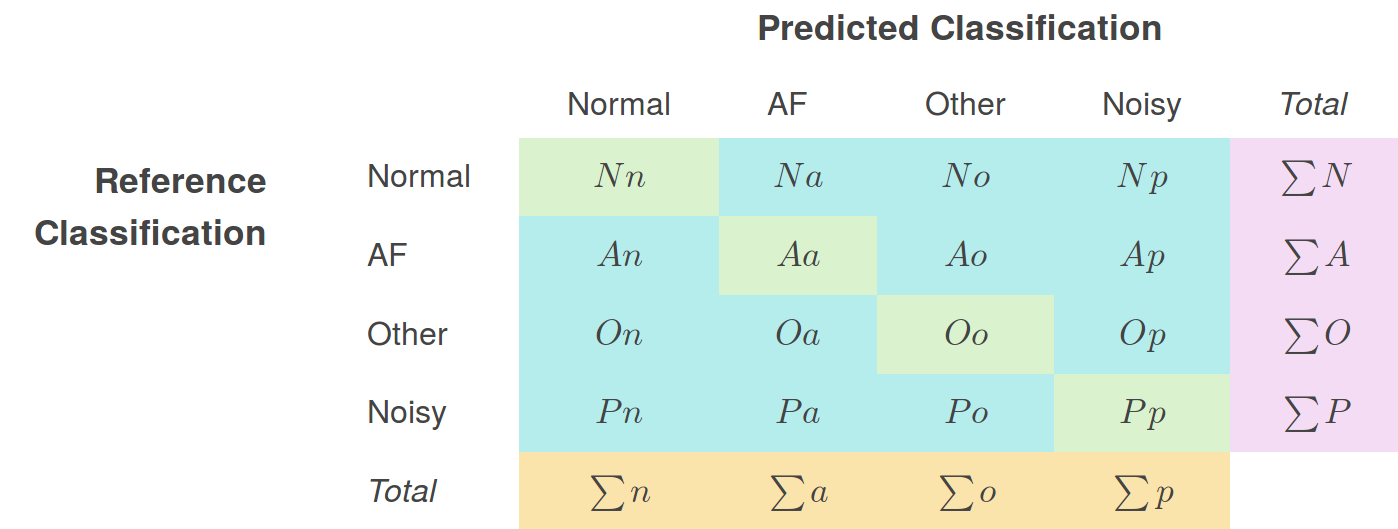
\includegraphics[width=.8\textwidth]{conf-mat-af}
  \caption{Confusion matrix. Diagonal values represent prediction \textbf{hit}, off-diagonals represent \textbf{miss}. Image credits AF Challenge 2017}
  \label{fig:FCN}
\end{figure}

\section{The training set}
In order to keep track of how well our model generalized the features, and to avoid over-fitting, the original downloaded samples were separated into three sets.
First we selected 20\% of every class to keep it as a \textbf{test} set.
As a next step, the remaining 80\% were fed to an augmentation algorithm that added additive and multiplicative noise sampled from normal distribution biased to match the moment of each individual sample, and re-sampled each class' randomly selected entries to make an even distribution between classes.
Finally the augmented data was separated into \textbf{train} and \textbf{evaluation} set in an 80-20 ratio.
We use evaluation set to keep track how our model performs on unseen data.
Different \textit{training policies} modify learning rate, perturb the network parameters, or early stopping when over-fit occurs for given number of consecutive iterations.

\section{Data standardization}
We experimented with different normalization techniques such as standard normalizing per sample, or with the global mean and average with no significant difference in the results
Our current experiments involve standardizing the samples by heart rate frequency, thus the class relevant invariance can be easier learned by the the network.

\paragraph{Toy problem.}
A simple example is the following: suppose we have two patients, one who drinks coffee regularly resulting in a high heart rate (even in healthy) and one who runs marathon every week with low heart rate at rest.
If both were having the same cardiac symptom probably the cardiologist would record their natural heart rate to have a baseline, a reference point to use for diagnosis.
This is because the time domain patterns are expressively specific to the patient's heart rate.
Technically this means, if the atrial fibrillation specific curve would appear in both samples it would probably appear elongated or compressed --- and the model had to learn both patterns as if no similarity would have exist between them.
This problem could lead to a case where the network would discard some rare feature, in order to reserve the capacity for the trivial pattern just with different lengths.

\paragraph{Solutions.}
To counterweight we could increase the capacity of the network, which often leads to significant improvement in performance on the train set, however at the same time as a by-product the performance on validation set decays, since the model is more likely to over-fit, simply remember the train samples, and loses its ability to generalize well.
The loss is likely to happen since our training set only contains less than 8K samples.
An other solution is standardizing the heart rate frequency of our samples by resizing the whole sequence in time, which would in case, solve our toy example.
We made sure that discarding the sample specific frequency has no significant relevance to the corresponding class. For details of class BPM variance see Figure \ref{fig:violin}


\begin{figure}[h]
  \centering
  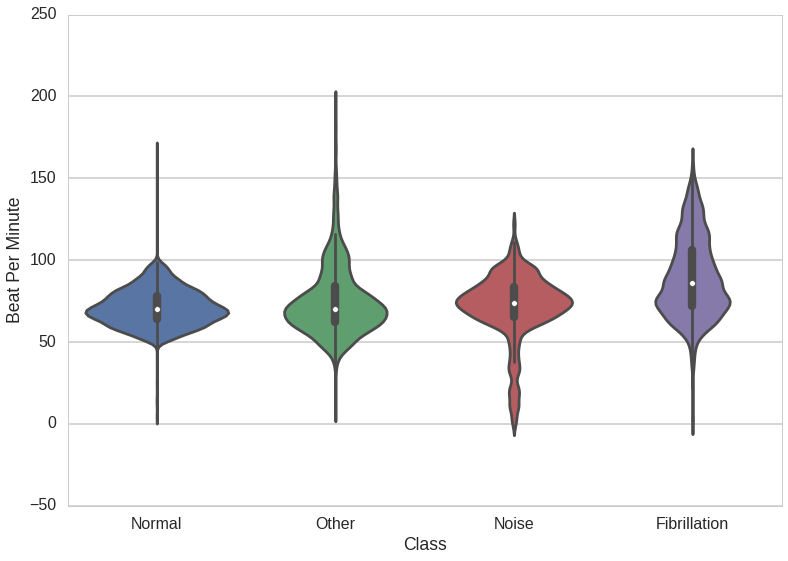
\includegraphics[width=\textwidth]{bpm_violin}
  \caption{The heart rate distribution and variance between classes is similar (except of cases in Noise class where the heart beat detection algorithm fails to find the R waves, thus resulting in extreme values, which we intend to filter before the entry reaches the valid sample classifiers), so discarding the average heart rate by normalizing every sample by the value, presumably would not affect negatively the performance of our network.}
  \label{fig:violin}
\end{figure}


\section{Regularization}

\paragraph{Weighted loss.}
Our first attempts to improve accuracy on rare samples was to set higher loss on underrepresented classes to encourage the network to optimize by learning to recognize these samples better, but it resulted in over-fitting and soon was replaced by augmented evenly distributed mini-batches.
\textit{Mini-batch} is a common method throughout almost every Deep Learning algorithm.
It enables the back-end to train the network with multiple samples at once.
Both parallel inference and weight adjusting is implemented in the latest machine learning frameworks.

\paragraph{Default optimizer, and other regularization.}
We are using the current state-of-the art optimizer algorithm ADAM~\cite{kingma_adam:_2014} and DropConnect~\cite{wan_regularization_2013} with $p=0.5$ settings. We also apply weight decay, by adding $L_2$ norm of each $\theta$ in the networks parameters to the overall loss function and use soft labels (perturbed one-hot vectors) in order to prevent the networks from favoring a specific class.
Our training policy varies over different settings, currently we are using early stopping method: after 10 consecutive steps where validation performance have not been improved the trainer shuts down, to enable other train routines use the allocated device --- otherwise the models are evaluated after a previously given number of steps. Throughout the training, we decrease exponentially the learning rate, in order to prevent the model from oscillation.
